\documentclass[border=10pt]{standalone}
\usepackage{tikz}
\usetikzlibrary{shapes.geometric, arrows.meta, positioning, calc, fit, backgrounds, shadows.blur, decorations.pathreplacing}
\usepackage[T1]{fontenc}
\usepackage{helvet}
\renewcommand{\familydefault}{\sfdefault}

\definecolor{morphorange}{HTML}{FF6B2B}
\definecolor{morphdark}{HTML}{0D0D1A}
\definecolor{morphgray}{HTML}{1A1A2E}
\definecolor{morphblue}{HTML}{4A90D9}
\definecolor{morphpurple}{HTML}{8B5CF6}
\definecolor{morphgreen}{HTML}{10B981}
\definecolor{morphaccent}{HTML}{F59E0B}
\definecolor{textwhite}{HTML}{F0F0F0}
\definecolor{textgray}{HTML}{9CA3AF}
\definecolor{cardbg}{HTML}{16162A}
\definecolor{layerbg1}{HTML}{1E1E3A}
\definecolor{layerbg2}{HTML}{1A1A30}
\definecolor{layerbg3}{HTML}{161628}
\definecolor{layerbg4}{HTML}{121222}

\begin{document}
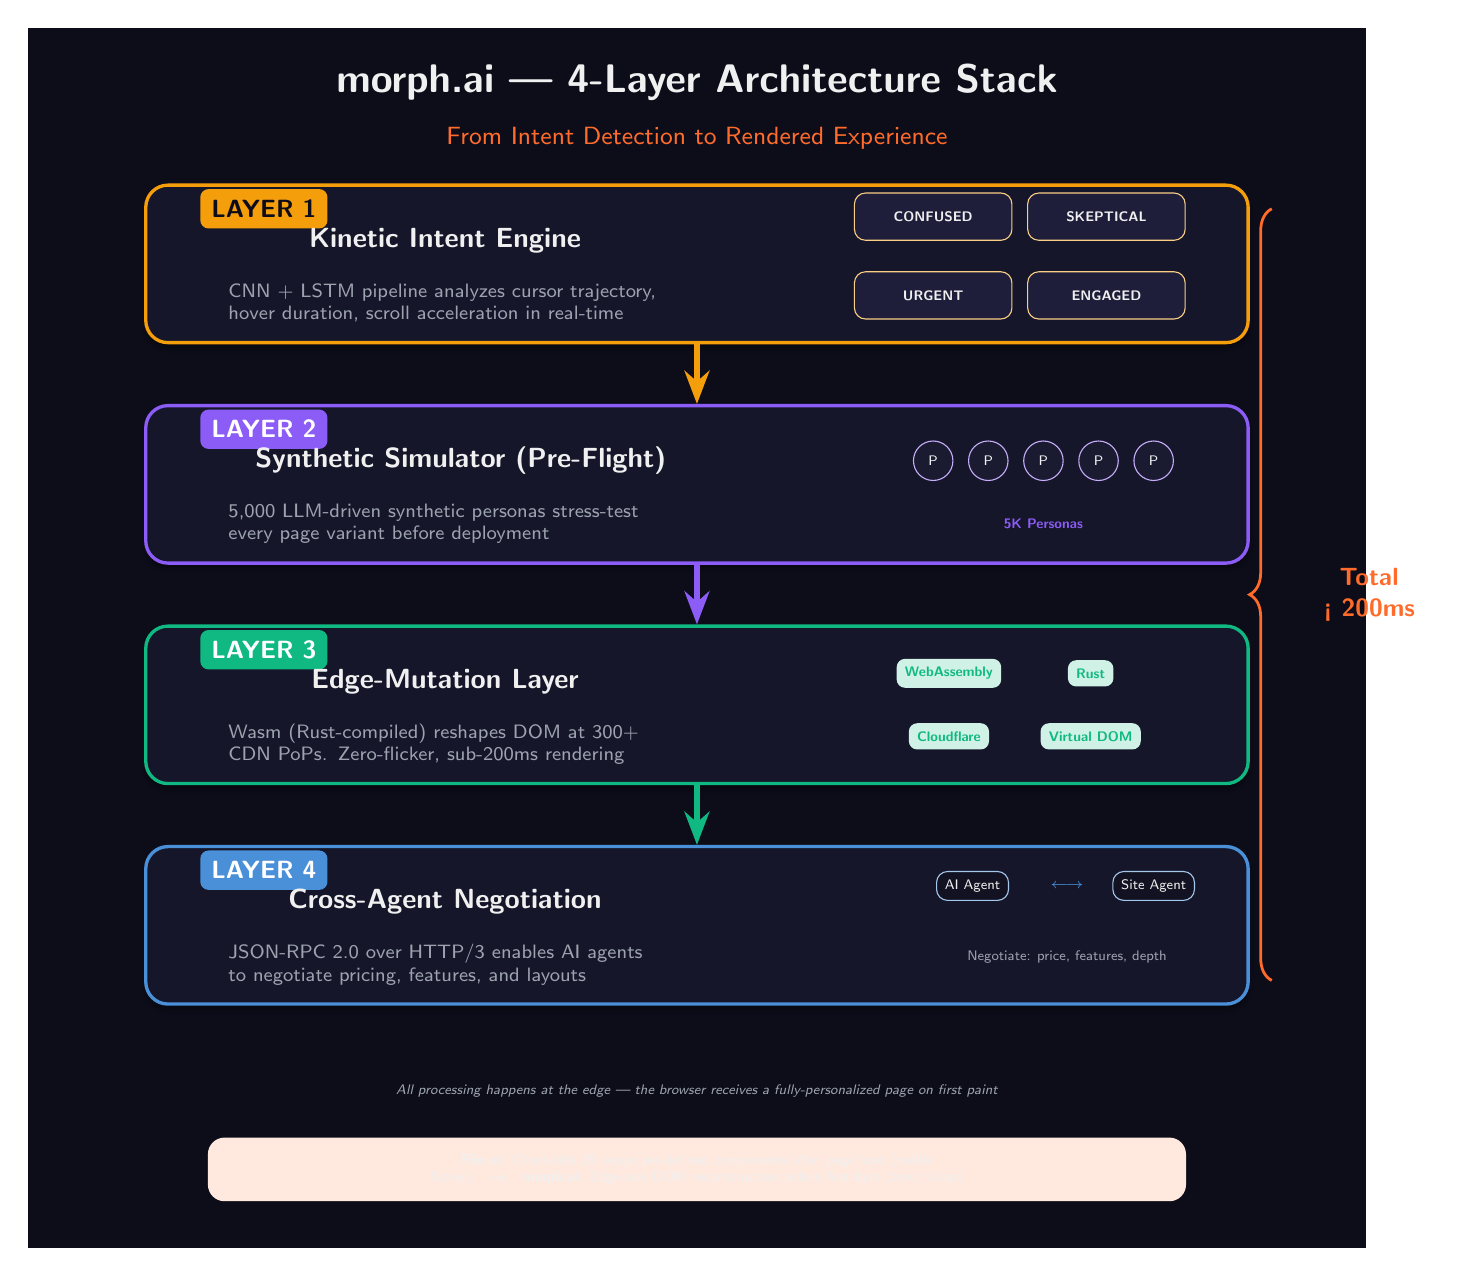
\begin{tikzpicture}[
    every node/.style={font=\sffamily},
    >=Stealth,
    layer/.style={draw=#1, fill=cardbg, rounded corners=8pt, minimum width=14cm, minimum height=2cm, 
                  line width=1.2pt, blur shadow={shadow blur steps=5, shadow xshift=0pt, shadow yshift=-2pt}},
]

% Background
\fill[morphdark] (-8.5,-10.5) rectangle (8.5,5);

% Title
\node[text=textwhite, font=\sffamily\bfseries\Large] at (0,4.3) {morph.ai — 4-Layer Architecture Stack};
\node[text=morphorange, font=\sffamily\small] at (0,3.6) {From Intent Detection to Rendered Experience};

% === LAYER 1: Kinetic Intent Engine ===
\node[layer=morphaccent] (L1) at (0, 2) {};
\node[fill=morphaccent, rounded corners=3pt, text=morphdark, font=\sffamily\bfseries\small, inner sep=4pt] 
      at (-5.5, 2.7) {LAYER 1};
\node[text=textwhite, font=\sffamily\bfseries] at (-3.2, 2.3) {Kinetic Intent Engine};
\node[text=textgray, font=\sffamily\scriptsize, text width=5.5cm] at (-3.2, 1.5) 
      {CNN + LSTM pipeline analyzes cursor trajectory, hover duration, scroll acceleration in real-time};

% Layer 1 detail boxes
\node[draw=morphaccent!50, fill=layerbg1, rounded corners=4pt, minimum width=2cm, minimum height=0.6cm,
      text=textwhite, font=\sffamily\tiny\bfseries] (s1) at (3, 2.6) {CONFUSED};
\node[draw=morphaccent!50, fill=layerbg1, rounded corners=4pt, minimum width=2cm, minimum height=0.6cm,
      text=textwhite, font=\sffamily\tiny\bfseries] (s2) at (5.2, 2.6) {SKEPTICAL};
\node[draw=morphaccent!50, fill=layerbg1, rounded corners=4pt, minimum width=2cm, minimum height=0.6cm,
      text=textwhite, font=\sffamily\tiny\bfseries] (s3) at (3, 1.6) {URGENT};
\node[draw=morphaccent!50, fill=layerbg1, rounded corners=4pt, minimum width=2cm, minimum height=0.6cm,
      text=textwhite, font=\sffamily\tiny\bfseries] (s4) at (5.2, 1.6) {ENGAGED};

% === LAYER 2: Synthetic Simulator ===
\node[layer=morphpurple] (L2) at (0, -0.8) {};
\node[fill=morphpurple, rounded corners=3pt, text=white, font=\sffamily\bfseries\small, inner sep=4pt] 
      at (-5.5, -0.1) {LAYER 2};
\node[text=textwhite, font=\sffamily\bfseries] at (-3, -0.5) {Synthetic Simulator (Pre-Flight)};
\node[text=textgray, font=\sffamily\scriptsize, text width=5.5cm] at (-3.2, -1.3) 
      {5,000 LLM-driven synthetic personas stress-test every page variant before deployment};

% Persona icons
\foreach \x in {3, 3.7, 4.4, 5.1, 5.8} {
    \node[draw=morphpurple!50, fill=layerbg2, circle, minimum size=0.5cm, text=textwhite, font=\tiny] at (\x, -0.5) {P};
}
\node[text=morphpurple, font=\sffamily\tiny\bfseries] at (4.4, -1.3) {5K Personas};

% === LAYER 3: Edge-Mutation Layer ===
\node[layer=morphgreen] (L3) at (0, -3.6) {};
\node[fill=morphgreen, rounded corners=3pt, text=white, font=\sffamily\bfseries\small, inner sep=4pt] 
      at (-5.5, -2.9) {LAYER 3};
\node[text=textwhite, font=\sffamily\bfseries] at (-3.2, -3.3) {Edge-Mutation Layer};
\node[text=textgray, font=\sffamily\scriptsize, text width=5.5cm] at (-3.2, -4.1) 
      {Wasm (Rust-compiled) reshapes DOM at 300+ CDN PoPs. Zero-flicker, sub-200ms rendering};

% Tech badges
\node[fill=morphgreen!20, rounded corners=3pt, text=morphgreen, font=\sffamily\tiny\bfseries, inner sep=3pt] 
      at (3.2, -3.2) {WebAssembly};
\node[fill=morphgreen!20, rounded corners=3pt, text=morphgreen, font=\sffamily\tiny\bfseries, inner sep=3pt] 
      at (5, -3.2) {Rust};
\node[fill=morphgreen!20, rounded corners=3pt, text=morphgreen, font=\sffamily\tiny\bfseries, inner sep=3pt] 
      at (3.2, -4.0) {Cloudflare};
\node[fill=morphgreen!20, rounded corners=3pt, text=morphgreen, font=\sffamily\tiny\bfseries, inner sep=3pt] 
      at (5, -4.0) {Virtual DOM};

% === LAYER 4: Cross-Agent Negotiation ===
\node[layer=morphblue] (L4) at (0, -6.4) {};
\node[fill=morphblue, rounded corners=3pt, text=white, font=\sffamily\bfseries\small, inner sep=4pt] 
      at (-5.5, -5.7) {LAYER 4};
\node[text=textwhite, font=\sffamily\bfseries] at (-3.2, -6.1) {Cross-Agent Negotiation};
\node[text=textgray, font=\sffamily\scriptsize, text width=5.5cm] at (-3.2, -6.9) 
      {JSON-RPC 2.0 over HTTP/3 enables AI agents to negotiate pricing, features, and layouts};

% Protocol flow
\node[draw=morphblue!50, fill=layerbg4, rounded corners=4pt, text=textwhite, font=\sffamily\tiny, inner sep=3pt] 
      (bot) at (3.5, -5.9) {AI Agent};
\node[text=morphblue, font=\sffamily\tiny\bfseries] at (4.7, -5.9) {$\longleftrightarrow$};
\node[draw=morphblue!50, fill=layerbg4, rounded corners=4pt, text=textwhite, font=\sffamily\tiny, inner sep=3pt] 
      (site) at (5.8, -5.9) {Site Agent};
\node[text=textgray, font=\sffamily\tiny] at (4.7, -6.8) {Negotiate: price, features, depth};

% === Vertical flow arrows ===
\draw[->, morphaccent, line width=2pt] (L1.south) -- (L2.north);
\draw[->, morphpurple, line width=2pt] (L2.south) -- (L3.north);
\draw[->, morphgreen, line width=2pt] (L3.south) -- (L4.north);

% === Right-side latency annotations ===
\draw[decorate, decoration={brace, amplitude=8pt, mirror}, morphorange, line width=1pt] 
      (7.3, 2.7) -- (7.3, -7.1) node[midway, right=10pt, text=morphorange, font=\sffamily\small\bfseries, text width=1.5cm, align=center] 
      {Total\\< 200ms};

% === Bottom ===
\node[text=textgray, font=\sffamily\tiny\itshape] at (0, -8.5) 
      {All processing happens at the edge — the browser receives a fully-personalized page on first paint};

% Comparison callout
\node[fill=morphorange!15, rounded corners=6pt, text=textwhite, font=\sffamily\tiny, inner sep=6pt, text width=12cm, align=center] 
      at (0, -9.5) 
      {\textbf{Fibr.ai:} Client-side JS swaps pre-defined components after page load (visible flicker)  \quad\textbf{→}\quad  
       \textbf{morph.ai:} Edge-side DOM reconstruction before first byte (zero flicker)};

\end{tikzpicture}
\end{document}
